\chapter{Implementierung}

\section{Einleitung}

Ziel dieser Arbeit war es, eine Simulationsumgebung für Sensorknoten zu schaffen. Es sollte viele verschiedene Arten von Sensorknoten geben, die jeweils einen oder mehrere verschiedene Sensoren besitzen. Mit diesen Knoten sollte ein Netzwerk aufgebaut werden, um die Umgebungsparameter eines Gebietes zu erfassen.
Die Daten der Simulation sollten visualisiert und ausgewertet werden.

\section{Aufbau und Struktur}

\subsection{Klassenübersicht}

Die Klassenübersichten wurden teilweise mit Hilfe von doxygen\cite{doxygen} erstellt. 

\begin{center}
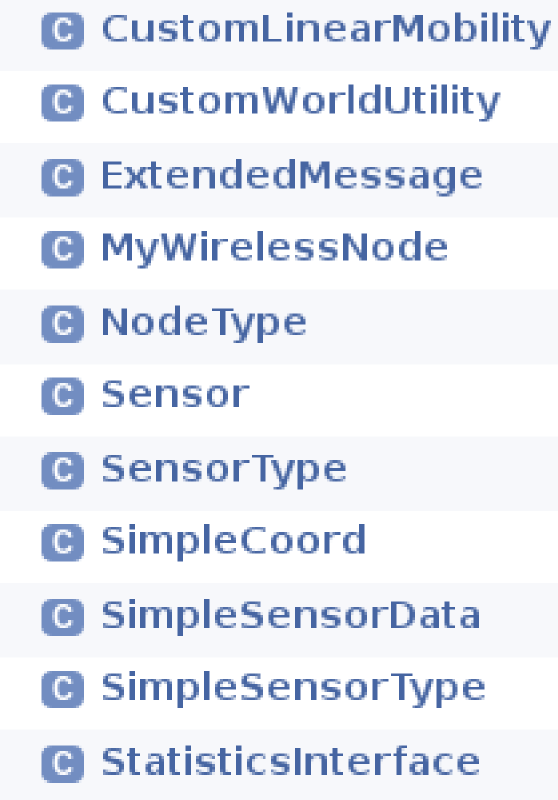
\includegraphics{Klassenuebersicht}
\end{center}

\paragraph{CustomLinearMobility}

\begin{center}
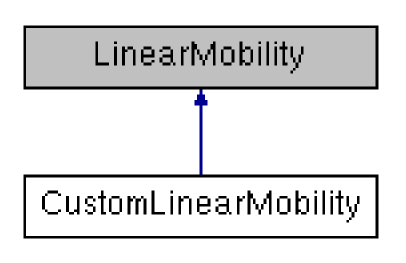
\includegraphics{CustomLinearMobility}
\end{center}

Diese Klasse erbt direkt von der in MiXiM definierten LinearMobility. Sie ist um einige Parameter erweitert, die es ermöglichen, dass die Knoten beschleunigen können und eine maximale Geschwindigkeit \textbf{maxSpeed} erreichen, sollte eine definiert sein.
Der Parameter \textbf{maxSpeed} kann ebenso auf 0 gesetzt werden, um die Knoten von mobil in stationär umzuwandeln.

\paragraph{CustomWorldUtility}

Die Klasse CustomWorldUtility ist eine der wichtigsten für die Simulation. Sie repräsentiert den \textbf{Playground}, also den Bereich indem sich die Knoten befinden. Sie erbt von der Klasse BaseWorldUtility aus dem MiXiM-Framework. BaseWorldUtility stellt die nötigen Funktionalitäten für den Playground bereit. \newline

\begin{center}
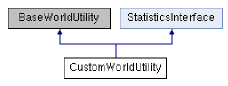
\includegraphics{CustomWorldUtility1}
\end{center}

Zusätzlich dazu stellt die Klasse selbst die notwendigen Parameter für die Umwelt bereit. Nach dem Starten der Simulation steht darin jeweils ein zweidimensionales Array pro Sensortyp bereit: temperatureArray, pressureArray, humidityArray und lightArray. Diese enthalten die Parameter der Umgebung; temperatureArray beinhaltet zum Beispiel, wie der Name schon sagt, Informationen über die Temperatur. \newline
Es kann zu Beginn der Simulation entschieden werden, ob neue Werte berechnet werden sollen oder die bereits vorhandenen Werte für die Umgebung übernommen werden sollen. Die Arrays besitzen die gleiche Größe wie der Playground. Diese Größe ist auch zusätzlich in den Parametern sizeX und sizeY gespeichert.

\begin{center}
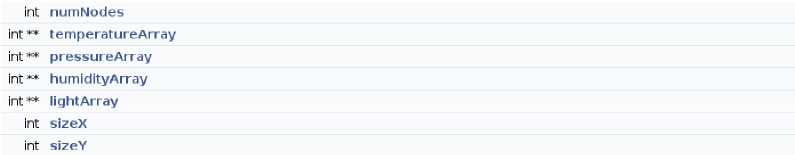
\includegraphics[width=\textwidth]{CustomWorldUtility3}
\end{center}

Zum Erstellen neuer Daten kann die Funktion \textbf{generateEnvironmentData()} genutzt werden. Es ist dadurch auch möglich während der Simulation neue Werte zu generieren, indem man diese Funktion aufruft. Die Funktion legt pro Umweltparameter eine xml-Datei im Ordner \textit{WorldModel/data} an. Jede der xml-Dateien wird beim Start mit Hilfe der Funktion \textbf{readXML(int)} eingelesen, verarbeitet, also in ein Array umgewandelt und anschließend in der Klasse gespeichert. \newline
Sollte nun ein Sensor nach dem Wert an seiner aktuellen Position fragen, so kann diese Klasse mit Hilfe der Funktionen \textbf{generateMessage(const char*)} und \textbf{sendSensorResponse(std::string, cGate *)} eine Antwort generieren. Die Position kann dabei mit der Klasse \textbf{SimpleCoord} und der Wert an dieser Position mit \textbf{SimpleSensorData} repräsentiert und per Nachricht verschickt werden.

\begin{center}
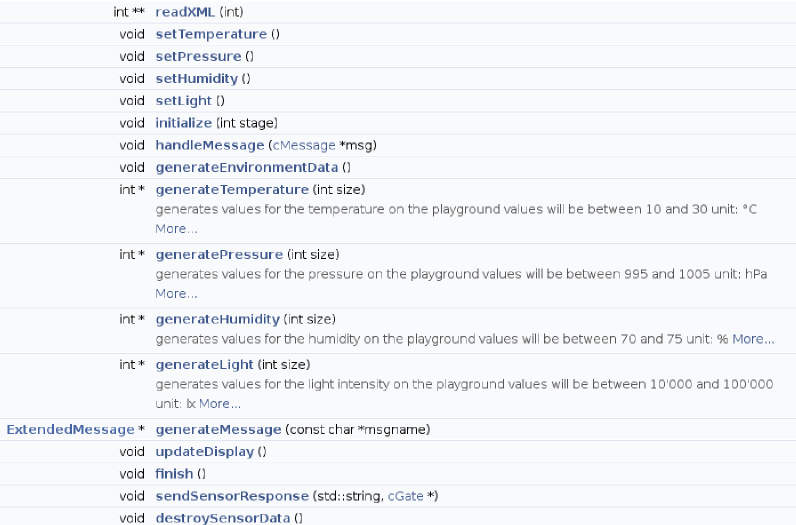
\includegraphics[width=\textwidth]{CustomWorldUtility2}
\end{center}

\paragraph{ExtendedMessage}

ExtendedMessage erbt direkt von der Klasse cMessage, der Standard-Nachrichtenklasse in Omnet++. Im Grunde stellt cMessage alle benötigten Funktionen bereit. ExtendedMessage ist nur aus dem Grund vorhanden, um zusätzliche Statistiken über Nachrichten erstellen zu können, zum Beispiel wie oft eine einzelne Nachricht weitergesendet wurde.

\begin{center}
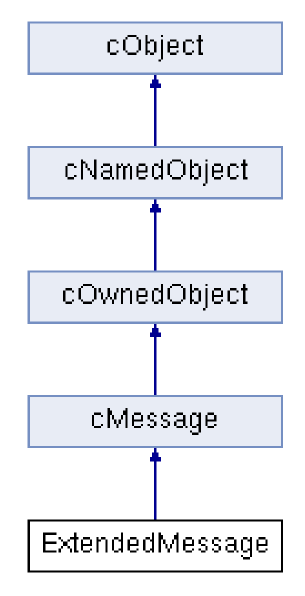
\includegraphics{ExtendedMessage}
\end{center}

\paragraph{MyWirelessNode und Sensor}

MyWirelessNode implementiert das StatisticsInterface und erbt von der Klasse Sensor, welche vom cSimpleModule erbt. Die Klasse Sensor soll lediglich mehr Struktur in die Klasse MyWirelessNode bringen und die Funktionen und Attribute in jene unterteilen, welche für die allgemeine Kommunikation und weiteres verantwortlich sind und jene, die nur für die Sensordaten zuständig sind. \newline

\begin{center}
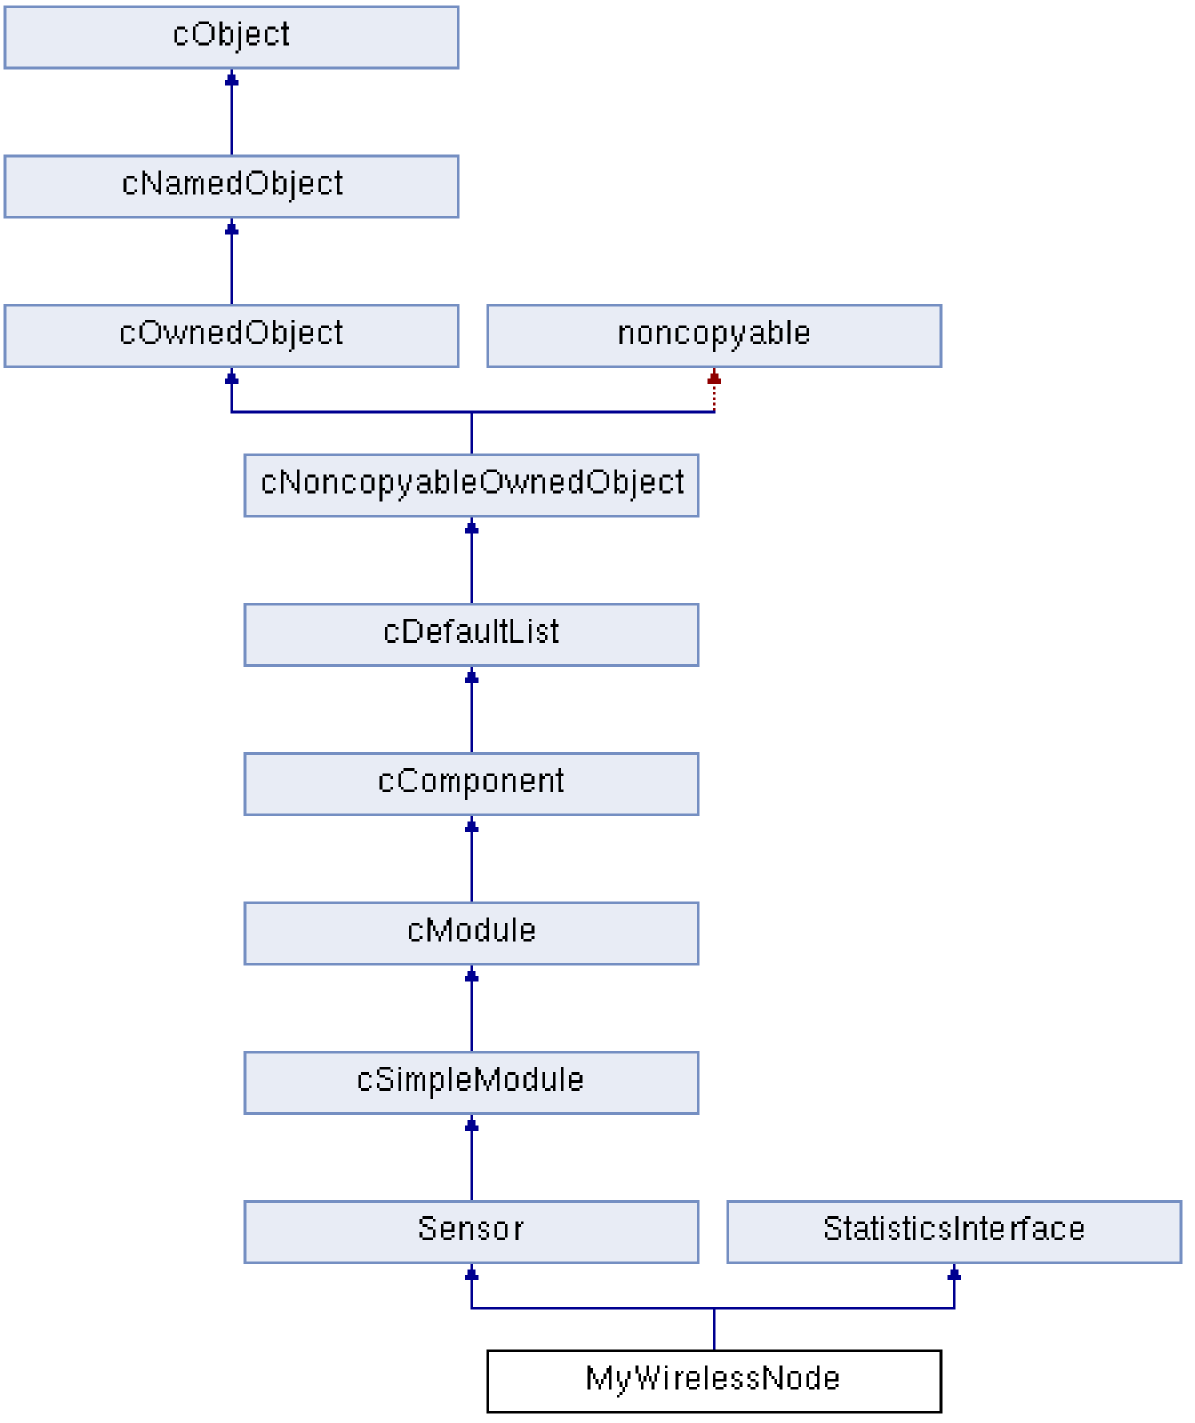
\includegraphics{MyWirelessNode}
\end{center}

Es ist neben der Klasse für die Umwelt CustomWorldUtility die zweite essentielle Klasse der Simulation. Das Verhalten aller Knoten im Netzwerk wird durch MyWirelessNode definiert. Neben den Standardfunktionen eines Omnet++-Moduls, \textbf{initialize()}, \textbf{handleMessage()} und \textbf{finish()}, können Knoten zum Beispiel ihre Position abfragen. \newline
Dazu dient die Funktion \textbf{updatePosition()}, welche das Attribut \textbf{position} aktualisiert. Des weiteren beinhaltet das Modul Funktionen zum Anfordern von Umweltdaten. Dies erfolgt über einen GET request an das World-Modul, welches anschließend eine Antwort darauf sendet.

\paragraph{NodeType}

\begin{center}
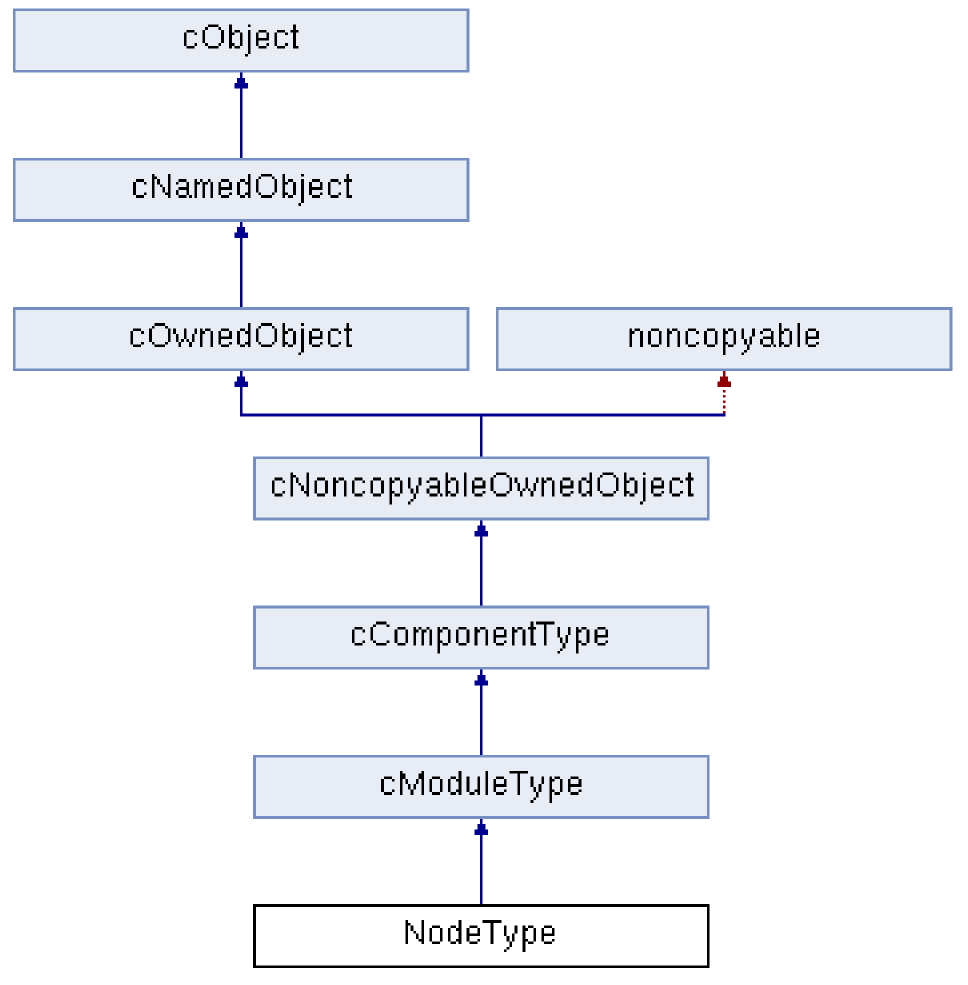
\includegraphics{NodeType}
\end{center}

NodeType erbt von der Klasse cModuleType und erfüllt den gleichen Zweck. Es ist dazu da die MyWirelessNode-Klassen für jeden Knoten anzulegen, sodass diese global bekannt sind, verwendet werden können und am Ende der Simulation wieder gelöscht werden.

\paragraph{SensorType}

\begin{center}
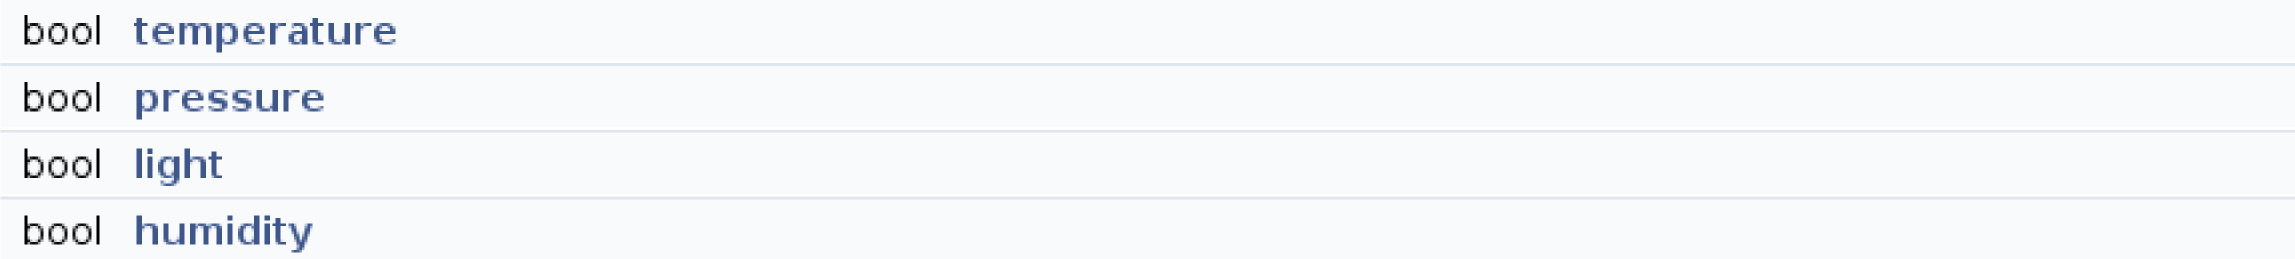
\includegraphics{SensorType}
\end{center}

Die Klasse SensorType ist eine Helferklasse für MyWirelessNode. Es besitzt lediglich 4 Attribute, welche definieren ob der jeweilige Knoten einen bestimmten Typ von Sensor besitzt oder nicht.

\paragraph{Simple*}

\begin{center}
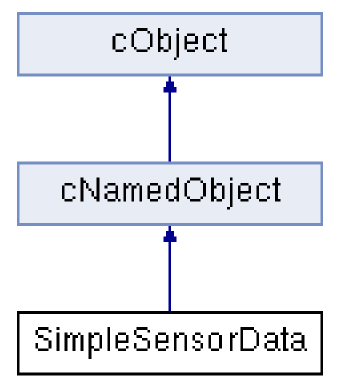
\includegraphics{SimpleClasses}
\end{center}

Es gibt die 3 Klassen SimpleCoord, SimpleSensorData und SimpleSensorType.  Sie erben jeweils direkt von cNamedObject und beinhalten nur wenige Attribute. So enthält SimpleCoord beispielsweise 3 Attribute x, y und z, um Koordinaten zu repräsentieren.\newline
cNamedObject und ebenso Kinderklassen davon lassen sich per leicht cMessage übertragen. Alle haben daher den Zweck eine einfache Kommunikation zu ermöglichen. So wird beispielsweise SimpleCoord benutzt, um beim Anfordern von Sensordaten in MyWirelessNode die Koordinaten an die CustomWorldUtility mit zu übertragen, damit in der Response der jeweilige Datensatz der richtigen Position zurückgegeben wird.

\paragraph{StatisticsInterface}

Dieses Interface enthält grundlegende Attribute für Statistiken. Klassen die dieses implementieren speichern somit zum Beispiel wie viele Nachrichten sie empfangen oder gesendet haben.

\subsection{Netzwerk}

Im folgenden Abschnitt werden alle Simulationsobjekte erläutert, also all jene, die durch die Sprache NED beschrieben wurden:

\begin{itemize} 
\item Simple Module
\begin{multicols}{2}
\begin{itemize}
\item CustomLinearMobility
\item CustomWorldUtility  
\item HumiditySensor
\item LightSensor
\item PressureSensor
\item Sensor
\item TemperatureSensor 
\end{itemize}
\end{multicols}
\item Compound Module
\begin{multicols}{2}
\begin{itemize}
\item HLNode
\item HLPNode
\item HNode
\item HPNode
\item LNode
\item LPNode
\item MyWirelessNode
\item PNode
\item THLNode
\item THLPNode
\item THNode
\item THPNode
\item TLNode
\item TLPNode
\item TNode
\item TPNode 
\end{itemize}
\end{multicols}
\begin{multicols}{2}
\item Networks
\begin{itemize}
\item MyNetwork
\end{itemize}
\item Messages
\begin{itemize}
\item ExtendedMessage
\end{itemize}
\end{multicols}
\end{itemize}

\subsubsection{Simple Module}

Simple Module sind Komponenten in einer Omnet++ Simulation, die die größte Auswirkung auf die Wirkungsweise des Netzwerkes haben. Das liegt daran, dass bei ihnen neben einer Beschreibung in NED auch eine Beschreibung in C++ vorliegt. Daher kann das Verhalten jener Module während der Simulation ausführlich definiert werden.

\paragraph{CustomLinearMobility}

Das Modul CustomLinearMobility ist eine Erweiterung der LinearMobility, welche MiXiM bereitstellt. Neben dem Verhalten welches in C++ beschrieben ist, ist das Modul lediglich um den Parameter maxSpeed erweitert, welcher in der omnetpp.ini definiert werden kann.

\paragraph{CustomWorldUtility}

Wie im Codebeispiel (\ref{lst:CustomWorldUtility}) zu sehen ist, ist das Modul CustomWorldUtility eine Erweiterung des Moduls BaseWorldUtility. Zusätzlich zu den darin definierten Eigenschaften hat es einige weitere Parameter. Zunächst eine bool'sche Variable, welche festlegt, ob zu Beginn der Simulation neue Umweltparameter generiert werden sollen. \newline Während numSensorNodes definiert, wieviele Sensorknoten im Netzwerk vorhanden sind und somit wieviele Gates zu Sensorknoten gehen, so definiert numGates die Anzahl der einzelnen Sensoren und somit auch die Anzahl der dahin gehenden notwendigen Gates. Da Sensorknoten auch mit mehr als einem Sensor bestückt sein können, ist der Wert beider Variablen mitunter durchaus verschieden.\newline
Die restlichen Variablen speichern die Umweltparameter in Form einer xml-Datei.

\begin{minipage}{\textwidth}
\begin{lstlisting}[language=ned,caption={CustomWorldUtility},label=lst:CustomWorldUtility]
package mynetwork.WorldModel;
import org.mixim.base.modules.BaseWorldUtility;

simple CustomWorldUtility extends BaseWorldUtility
{
    parameters:
        bool createData;
        int numGates;
        int numSensorNodes;
        xml xmlTemperature = xmldoc("WorldModel/data/temperature.xml");
        xml xmlPressure = xmldoc("WorldModel/data/pressure.xml");
        xml xmlHumidity = xmldoc("WorldModel/data/humidity.xml");
        xml xmlLight = xmldoc("WorldModel/data/light.xml");
        
        @class("CustomWorldUtility");
    gates:
        inout worldDataGate[numGates];
        inout toNode[numSensorNodes];
}
\end{lstlisting}
\end{minipage}

Neben den Parametern besitzt dieses Modul auch noch zusätzlich 2 verschiedene Arten von inout-Gates. Die Menge von worldDataGates verbindet die Welt mit jedem Sensor der auf einem Sensorknoten verbaut ist. Die Menge der toNode-Gates dient für die direkte Verbindung zwischen World und Nodes.

\paragraph{Sensoren}

Es gibt 5 Module welche die Sensoren definieren. Zum einen den allgemeinen Sensor, der das Vatermodul für alle 4 Sensortypen bildet. Er enthält nicht viel, lediglich Gates für Verbindungen zur Welt, um die Umweltparameter abfragen zu können und zum jeweiligen Knoten, für die Kommunikation innerhalb des Bauteils. Weiterhin besitzt er noch einen Parameter, der im Kindmodul den Typ des Sensors beschreibt.

\begin{multicols}{2}
\begin{itemize}
\item HumiditySensor
\item LightSensor
\item PressureSensor
\item TemperatureSensor
\end{itemize}
\end{multicols}

Die 4 Sensortypen, welche vom allgemeinen Sensor erben, definieren jeweils nur den Typ des Sensors. Sie können auf den Knoten als Submodule verwendet werden und somit 15 verschiedene Sensorknoten bilden.

\begin{minipage}{\textwidth}
\begin{lstlisting}[language=ned,caption={Sensor},label=lst:Sensor]
package mynetwork.Node.Sensor;

simple Sensor 
{
    parameters:
        //type of the sensor
        string type;
	    @display("i=block/wrx");
	    @class("Sensor");
	gates: 
	    inout toNode;
	    inout worldDataGate;
}
\end{lstlisting}
\end{minipage}

\subsubsection{Compound Module}

Compound Module dienen dazu, andere Module zusammenzufassen, sollen jedoch keine eigene aktive Funktionalität definieren. Ihr Verhalten soll sich allein durch die Submodule ergeben. Es ist daher nicht sinnvoll eine C++-Klasse für diese Module zu definieren.\newline
Alle Sensorknoten, die in dieser Simulation vorkommen sind solche Compound Module.

\paragraph{MyWirelessNode}



\paragraph{Sensorknoten}

\subsubsection{Networks}

\paragraph{MyNetwork}

\subsubsection{Messages}

\paragraph{ExtendedMessage}

\section{Funktionsweise}

was funktioniert wie
was wurde überhaupt umgesetzt
was fehlt evtl/verbesserungsideen